\documentclass[border=10pt]{standalone}

\usepackage{tikz}
\usepackage{tikzsymbols}
\usetikzlibrary{calc,patterns,shapes.geometric}

\def\centerarc[#1](#2)(#3:#4:#5){\draw[#1] ($(#2)+({#5*cos(#3)},{#5*sin(#3)})$) arc (#3:#4:#5);}

\begin{document}
	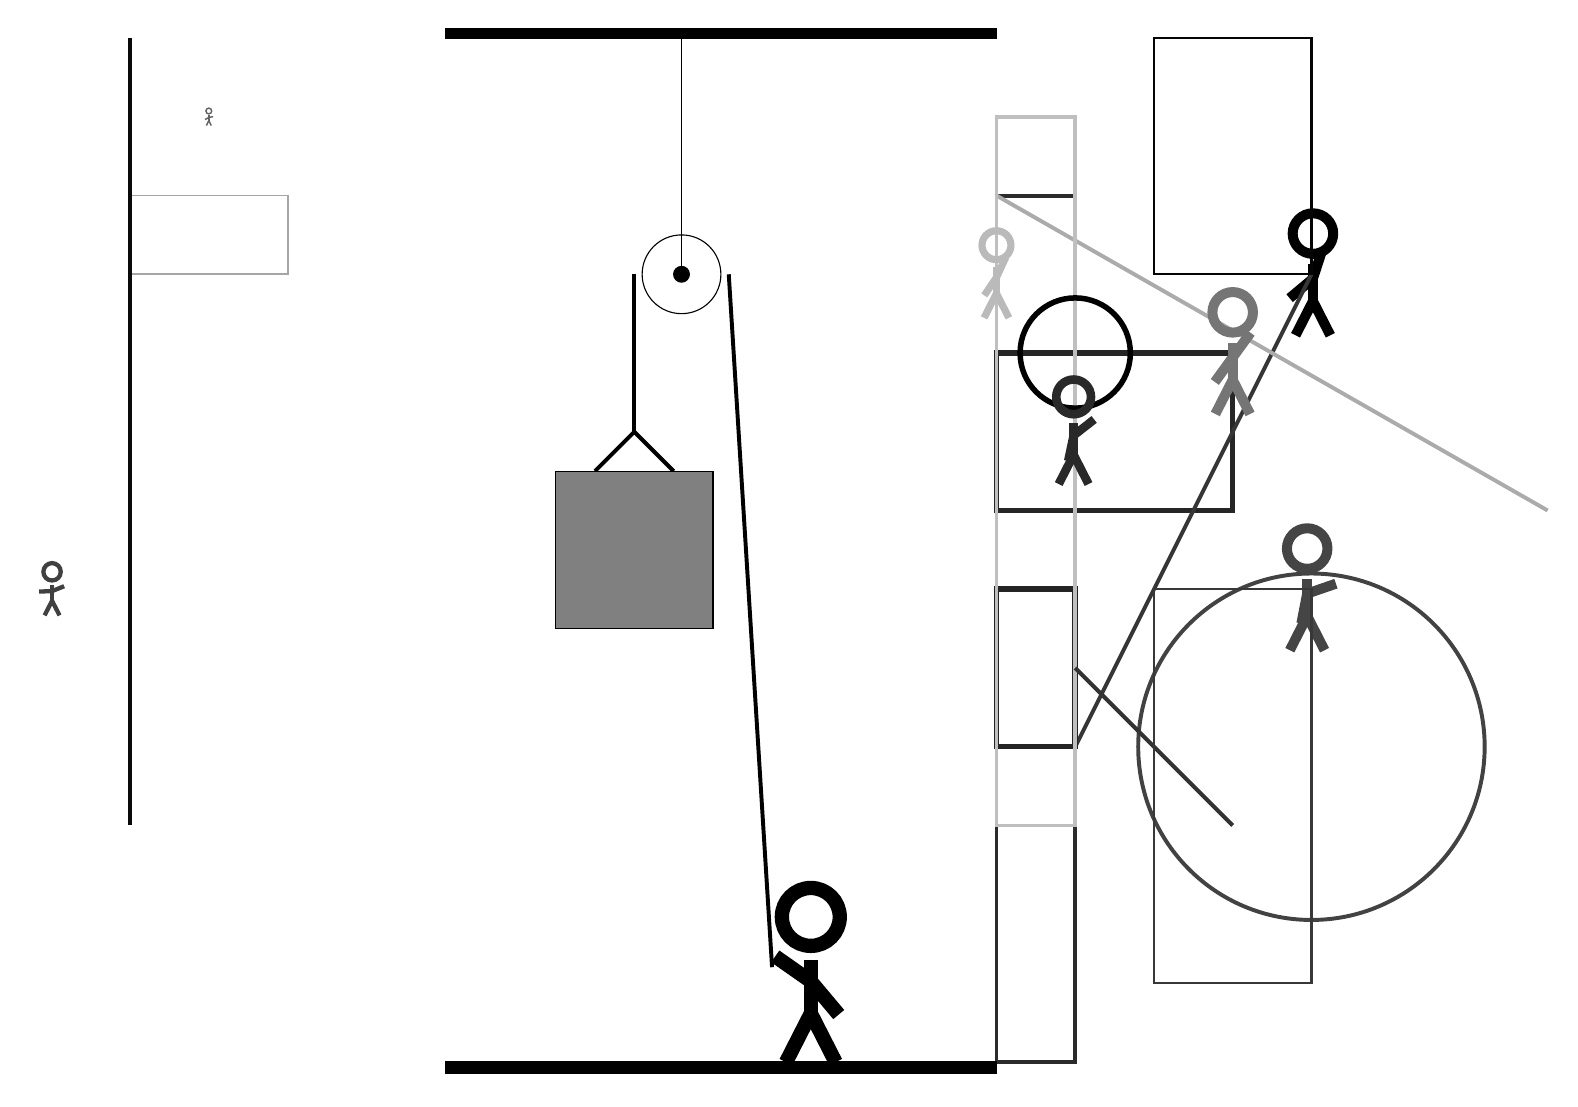
\begin{tikzpicture}
		%%%%% START %%%%%
		
		\draw[fill=black] (-2, 10) rectangle (5, 10.125);
		
		\draw (1, 7) circle (0.5);
		\draw[fill=black] (1, 7) circle (0.1);
		\draw (1, 10) -- (1, 7);
		
		\draw[line width=0.5mm] (-0.1, 4.5) -- (0.4, 5.0) -- (0.9, 4.5);
		\draw[fill=black!50] (-0.6, 4.5) rectangle (1.4, 2.5);
		
		\node[line width=0.3mm, color=black!100] at (9, 7) {\Strichmaxerl[7][40][72]};
		
		\draw[line width=0.7mm, color=black!85] (5, 6) rectangle (8, 4);
		\node[line width=0.2mm, color=black!75] at (-7, 3) {\Strichmaxerl[3][2][22]};
		\draw[line width=0.3mm, color=black!36] (5, 9) rectangle (5, 1);
		\draw[line width=0.5mm, color=black!79](9, 7) -- (6, 1);
		\draw[line width=0.5mm, color=black!83] (6, -3) rectangle (5, 8);
		\draw[line width=0.2mm, color=black!35] (-4, 7) rectangle (-6, 8);
		
		\draw [line width=0.5mm, color=black!74](9, 1) circle (2.2);
		\draw[line width=0.7mm, color=black!86] (6, 3) rectangle (5, 1);
		
		\draw[line width=0.5mm, color=black!33](5, 8) -- (12, 4);
		
		\draw[line width=0.5mm, color=black!25] (5, 0) rectangle (6, 9);
		
		\draw[line width=0.5mm, color=black!80](6, 2) -- (8, 0);
		\node[line width=0.4mm, color=black!61] at (-5, 9) {\Strichmaxerl[1][30][10]};
		
		\node[line width=0.7mm, color=black!27] at (5, 7) {\Strichmaxerl[5][56][65]};
		\draw[line width=0.3mm, color=black!98] (7, 7) rectangle (9, 10);
		\node[line width=0.4mm, color=black!73] at (9, 3) {\Strichmaxerl[7][79][19]};
		
		\draw[line width=0.6mm, color=black!40] (-3, -2) rectangle (-3, -2);
		
		\draw[line width=0.5mm, color=black!96](-6, 10) -- (-6, 0);
		\draw[line width=0.3mm, color=black!78] (7, -2) rectangle (9, 3);
		\node[line width=0.4mm, color=black!54] at (8, 6) {\Strichmaxerl[7][54][54]};
		\draw [line width=0.7mm, color=black!100](6, 6) circle (0.7);
		
		\node[line width=0.3mm, color=black!84] at (6, 5) {\Strichmaxerl[6][78][38]};
		
		\draw[line width=0.5mm] (0.4, 7) -- (0.4, 5.0);
		\centerarc[line width=0.5mm](1, 7)(0:180:0.6);
		\draw[line width=0.5mm](1.6, 7) -- (2.15, -1.8);
		
		\node at (2.6, -1.9) {\Strichmaxerl[10][-35][-50]};
		
		\draw[fill=black] (-2, -3) rectangle (5, -3.15);
		
		%%%%% END %%%%%
	\end{tikzpicture}
\end{document}